\documentclass[10pt]{article}
\raggedright
\parindent=1.5em
\usepackage{moreverb}
\usepackage{algorithmic}
\usepackage{setspace} 
\usepackage{graphicx}
\usepackage{url}

% Set Margins
\setlength{\textwidth}{6.5in}
\setlength{\oddsidemargin}{0in}
\hoffset=-.2in
\setlength{\textheight}{9.5in}
\setlength{\topmargin}{-1in}

\title{Automated Cut-Up Poem Generation from Large Corpora}
\author{Nathaniel K Smith}

\begin{document}

\maketitle

\begin{abstract}
This paper presents a new approach to computer poetry, presenting an algorithm
that performs a directed cut-up poem generation technique on a large corpus. The
technical implementation of the algorithm and its associated modules will be
discussed in detail. To provide background and motivation, a survey of existing
computer poetry generation techniques is presented with an analysis of their
ability to produce interesting results. To support my analysis, I offer a
discussion of how the technical implementation of computer poetry generation
affects the production of interesting results. I argue that the new, presented
algorithm fills both a technical and creative gap within the existing computer
poetry landscape. Finally, opportunities for further research are discussed.
\end{abstract}

\tableofcontents
\doublespacing

\section{Introduction}
Innovation in the field of computer generated poetry has been sluggish at best,
most likely because of the historically small intersection between poets and
programmers \cite{Hart96}. It seems that most attempts made at `good' computer
poetry (A metric which is arguably even less measurable than `good' poetry on
its own) often fall prey to one of two problems: one, leaving too much to the
computer, thus cutting out human spontanaeity and creativity or two, treating
the computer as a bland random number generator and using an over-abundance of
human-prepared content.

I posit that there is a way to synthesize these two extremes by exploiting
human content easily accessible via the Internet. Huge changes in both the
amount of content stored online and the continuing ease of access to such
content mean that there is a massive store of thoughts, emotions, humour,
tradgedy, and other elements of `good' poetry just waiting to be used as
inspiration for the computer-poet. To this end, I present an algorithm that
`cuts up' a given, large corpus (presumably harvested from the Internet) and
produces a poem according to some desired output parameters.

This paper will discuss in detail my implementation of the algorithm and its
associated modules. To provide background and motivation, a survey of existing
computer poetry generation techniques is presented with an analysis of their
ability to produce interesting results. To support my analysis, I offer a
discussion of how the technical implementation of computer poetry generation
affects the production of interesting results. I argue that the new, presented
algorithm fills both a technical and creative gap within the existing computer
poetry landscape. Finally, opportunities for further research are discussed.

\subsection{Background}
\subsubsection{Two Categories}
My research into existing work in the field of computer poetry revealed two
general categories of techniques; one, I called \emp{generative} and the other,
\emp{templatized}. The former category relies on some input text and an
algorithm to produce new works, while the latter relies on a pre-defined
grammatical (or semantic) template to produce work from scratch (in other
words, without any input text).  

To adapt the summation found in \cite{Hart96}, templatized computer poetry has
this general flow: a human programmer creates some kind of initial structure
(either semantic or grammatical) and uses it along with software to produce a
work. A generative approach to computer poetry, on the other hand, would
provide a program that acts as a filter of sorts that takes some initial
text--not necessarily written by the programmer designing the program--and
converts it into a new work. 

\subsubsection{Existing Projects}
Early attempts at computer poetry were templatized techniques. The earliest
documented approach was Auto-Beatnik, which churned out randomly rendered poems
using grammatical structures and a vocabulary of english words (nouns, verbs,
pronouns, and so forth).  It was not until 1984 that another serious attempt at
poetry generation was publicised with the release of a work by the program
RACTER called \emph{The Policeman's Beard is Half-Constructed}. At 66 pages,
\emph{Policeman's Beard} was a much larger effort than the handful of short
poems output by Auto-Beatnik. However, the generation process was essentially
the same idea: the program called upon built-in grammatical templates and a
large vocabulary of english words \cite{Chamb84}. Despite the 22 years between
these two projects, they both were, at their core, automated versions of the
popular game Mad Libs.

A more recent templatized technique is detailed in \cite{Manurung00} and
\cite{Manurung03}. This technique stochastically evolves a poem from a simple
phrase or set of simple phrases into an interesting poem using a set of
evaluation functions.

This approach is a wide ranging departure from RACTER. The technique, packaged
in software named McGonagall, relies on the manipulation of grammatical
information using a Lexicalized Tree Adjoining Grammar (LTAG). The LTAG is a
derivation tree; in other words, it itself does not describe the phrase
structure of a sentence. Instead, it describes operations performed on a set of
phrases. Each node of the LTAG is an elementary tree describing some phrase
structure and each edge labels the location at which a child node should be
inserted into its parent node. These LTAG structures serve as a kind of
template from which poems are derived. Potential solutions are evolved using
the LTAGs and evaluated for things like meter, rhyme, and semantics.

An early and basic generative approach is the Travesty Engine discussed in
\cite{Hart96}. This technique accepted an input text and reorganized it using a
Markov chain (a random generative process in which future states are selected
based only on the present state of the generation). Given some $n$, the
Travesty Engine reassembled an input text $t$ such that the result, $s$,
contained all the same $n$ length substrings in $t$. At $n = 1$ the program
simply shuffled the letters of $t$; but at about $n = 9$, $t$ begins to
resemble a grammatically correct rearrangment of the phrases in $s$. Thus, for
varying levels of $n$, new poetry could be produced from any input and this
basic algorithm without the need for any kind of external lexicon.

A recent technique, and one similar to the technique I am proposing, uses
Vector Space Modeling to produce Haiku using content found on blogs throughout
the Internet \cite{Wong08}. This method produces modern (in other words, not
strictly 5-7-5) Haiku poems using randomly accessed blog content. 

Before any utilization of blog data is used, a keyword lexicon is first built
using common Haiku terms. Using this lexicon, HTML output from a blog search
engine is parsed and sentences containing lexicon words are extracted and
converted into fragments according to English grammatical rules. Finally, longer
fragments are filtered out of the repository leaving only fragments of a length
suitable for use in Haiku.

Three keywords are randomly picked from the lexicon and used to further narrow
the sentence repository. The remaining fragments are then run through an
analysis stage in which sentence pairs are picked based on a vector
representation of their semantic similarity. Finally, the `best' three lines
are picked for the final Haiku, each one semantically involving one of the
three random keywords originally picked.

Another approach similar to my technique is the case based reasoning technique
developed in \cite{Gervas01}. This approach accepts prose sentences to be
converted to poetry. Largely, the process is generative, making grammatical
changes to the input sentence as well as word substitutions. The target output
is specified by some existing stanza of the desired form (ie, a haiku). An
important part of the process, however, is a vocabulary of words that may be
substituted into the original prose to achieve the desired poetic structure,
making this approach a combination of templatized and generative techniques. A
user must supply this vocabulary for each poem desired.

\subsection{Analysis}
Throughout the course of this research it became evident that a common problem in
computer poetry was simply the question: Why? templatized techniques tended to
rely almost exclusively on the human programmers designing the poetry
generation software; it seemed like the computer was little more than a set of
dice. In \cite{Manurung03}, where the templatized technique is taken to an
extreme, the semantic scope of the produced work is still strictly limited to
what humans provide in the LTAG collection. It seems like computer poetry like
this isn't contributing anything to the field that a human couldn't already do
by hand.

The CBR approach suffers from similar problems despite being a partially generative technique.
A large part of the creativity of the system depends on the words chosen for
the vocabulary used, meaning that a human must premeditate the content of
produced poems. Similarly, a human user must select the poetic verses used to
compare potential outputs to when generating a poem.

The question is easier to answer for generative techniques. The Travesty
Engine, for example, produces new arrangements of pieces that humans may never
think to produce. It can reveal new meaning in an existing piece through purely
aleatoric means. Similarly, in the VSM Haiku generator, the produced poetry can
describe the zeitgeist of the blogs it searches (something that even Google
struggles to do). Clearly this poetry was doing something that a human couldn't
do: revealing meaning hidden within existing human prose. However, I submit
that in the former example the rearrangement is too simple; it doesn't go far
enough and its results become predictable after a fashion. In the latter
example, the final Haiku bear too little resemblance to their source material
to really articulate any kind of underlying meaning to the reader.

\section{Directed Cut-up Technique}
Thus, I present a new generative technique inspired by the work of the poet and
author William Burroughs. This technique exploits the diversity and large
number of sentences found in large corpora--for example, Wikipedia, the online
articles of a newspaper, or online public domain books--by scanning the
sentences within them, profiling them, and then using them to populate a poem
based on rules input by a human user. Thus, the technique \emph{cuts up}, like
Burroughs \cite{wikiCutup}, some given corpus in order to produce a poetic
result. I argue that, given a large and varied enough corpus, this technique
produces interesting work, and present several features of the resulting pieces
that support this.

\subsection{Explication of Algorithm}
The technique is driven by a short algorithm  supported by several modules. It
is presented in pseudo-code in figure \ref{fig:algorithm}. The algorithm, given some corpus $C$
containing several thousands of lines of text, stores each sentence of the
corpus in a databse with associated syllabic and phonetic information. Using
any number of simple guidelines supplied by a user, it proceeds to construct a
poem using the sentences stored in the database. Should the algorithm be unable
to locate a sentence to satisfy some line of the desired poem--say, a sentence with
10 syllables containing the word \emph{aleatoric} and rhyming with the word
\emph{trumpet}--it \emph{weakens} the rule for that line, relaxing the criteria
used in the database lookup to find a sentence that at least closely resembles
one needed to meet the user's guidelines. Without this technique, termination
is not guaranteed; however, every rule eventually weakens to the trivial rule,
which is satisfied by any sentence.

\pagebreak
\onehalfspacing
\begin{figure}[here]
\begin{algorithmic}
\STATE Given some corpus $C$ and database handle $DB$
\STATE $L\gets$ normalize($C$)
\STATE insert($DB$, profile($L$))
\STATE $i \gets$ input()
\STATE $R \gets$ rulesParse($i$) \COMMENT{a list of lists of Rule objects}
\STATE $P \gets \emptyset$ \COMMENT{the output poem (a list of lines)}
\FOR{$r \in R$}
    \STATE $S \gets$ select($DB$, ruleSetToQuery($r$))
    \IF {not $S$}
        \WHILE {$r\prime \gets$ weaken($r\prime$)}
            \STATE $S\prime \gets$ select($DB$, ruleSetToQuery($r\prime$))
            \IF { $S\prime$ }
                \STATE $S \gets S\prime$
                \STATE break
            \ENDIF
        \ENDWHILE
    \ENDIF
    \STATE $s \gets$ random($S$)
    \STATE push($P, s$)
\ENDFOR
\STATE output($P$)
\end{algorithmic}
\caption{My algorithm}
\label{fig:algorithm}
\end{figure}
\doublespacing

\subsection{Technical Implementation}
The tools involved in the implementation of this algorithm were Perl
5.10\cite{perl} and SQLite3\cite{sqlite3}. Perl was chosen due to its rich
Lingua::EN repository which contains many modules for parsing, splicing, and
cleaning up English text. Used in the implementation of this algorithm were the
CPAN modules Splitter\cite{splitter}, Phoneme\cite{phoneme}, and
Syllable\cite{syllable} of the Lingua::EN namespace. SQLite3 was chosen for its
speed, in-RAM database feature and portability.

Despite initial concerns about the ability of an interpreted language to
process enough text in a short time, the implementation ended up with favorable
benchmarks. Producing 10 line poems with an AB rhyme scheme and 10 syllables
per line from a SQLite3 database containing .4 million sentences consistently
took between .2 and .4 seconds. Parsing a 1 million line corpus and inserting
it into a SQLite3 database took 2.5 hours. The former benchmark indicates that
the poem generation code will scale for larger corpora, but the latter shows
that refactoring or rewriting will be necessary to support multimillion line
corpora. All of this work was performed on a modern laptop running Ubuntu with
a consumer grade dual-core CPU and 1 gigabyte of RAM.

It is important to note that there are numerous opportunities for parallelism
in this project that could be included in future refactors. Corpus acquisition
and poem production are both embarassingly parallel operations; content can be
downloaded asynchronously in the former and in the latter, a process can be
spawned for each line of a poem-in-progress as no single line depends on any
other line.

All code developed for this project is licensed under version 2.0 of the
Artistic License and freely available at
\url{http://github.com/nathanielksmith/weltanschauung}.

\subsection{Corpus Acquisition}
A key component of this approach is the presence of a large corpus. Years ago,
before the Internet expanded to its current volumnuous state, it is unlikely
that any such corpus would be publicly and freely available. Now, one can
consider the publicly accessible areas of the Internet as one huge corpus with
smaller selections of Internet content as subsets of this corpus.

For initial testing and debugging, a digitized version of a dozen short stories
by Jorge Luis Borges was manually developed and employed.

For later testing and protyping, a selection of 3,700 books from Project
Gutenberg were scraped using an automated script. From these books, 1,000,000
lines of text (out of a total 7,000,000) were analyzed, producing 433,850
profiled sentences stored in a database for use.

A scrape of several thousand Wikipedia pages was attempted, but the content
proved to be too diverse (in terms of encoding and structure) to be parsed
without lots of additional overhead. The primary issues were UTF-8 encoding and
the vagaries of sidebars, tables of contents, and headers.

\subsection{Corpus Processing}
For each sentence found in the input corpus, the following details are stored in a database:
\singlespacing
\begin{enumerate}
\item line number
\item rhyme sound
\item syllable count
\item number of words
\item sentence text
\end{enumerate}
\doublespacing

The rhyme sound is determined through analyzing the phonetic representation of
the last word of the sentence. Lingua::EN::Phoneme, a Perl module based on the
CMU Pronouncing Dictionary, is used to break apart the word into its
constituent phonemes. Its rhyme sound is defined to be the final vowel sound of
the phoneme list followed by any number of consonant sounds. For instance,
since the phonemes of the word \emph{bear} is B, AO1, R, its rhyme sound is
represented as `AO1R' while \emph{bears} would be represented as `AO1RS'.

Syllables are also counted using the Lingua::EN::Phoneme module. The syllable
count of a word is defined to be the number of vowel sounds (in other words,
phonemes with a string representation of length 3) found in its phonetic
representation.

Unfortunately, relying on the CMU dictionary means that there are occasionally
words which are not profiled in the listing. For these words, no rhyme sound is
recorded. For syllable counting, the Perl module Lingua::EN::Syllable is fallen
back to, which employs an intelligent vowel count technique to produce syllable
counts with about 80\% accuracy\cite{syllable}.

The line number is used both as a primary key for the sentence's database
representation as well as for determining line proximity.

\subsection{Rules System}
Once a corpus database is ready, user inputted guidelines for the desired
output are parsed into a list of lists of Rule objects that are capable of
weakening themselves and producing SQL clauses to be used in a SELECT
statement.

\subsubsection{Rule Class}
Though not included in the algorithm's original design, it became clear that
the only way to properly organize the rule code was through an object oriented
approach. I designed a Rule class which keeps track of a `weakness' level--the
number of times the rule has been liberalized by the algorithm--and provides
functions for weakening the rule returning a SQL clause that describes the rule
in its current state.

Each rule object's get\_clause function returns SQL suitable for appending to a
SELECT statement's WHERE clause. For example, the unweakened SQL for a
Rule::Syllable object initialized with an argument of 5 would be
`(num\_syllables = 5)'. Thus, the ruleSetToQuery needs only iterate over the
rule objects for any line of the poem it's constructing and join each object's
get\_clause output with the string ` AND ' to result in a statement like:

\begin{verbatim}
SELECT sentence 
    FROM lines 
    WHERE (num_syllables = 5) 
    AND (end_rhyme_sound = 'AO1') 
    AND (sentence LIKE '% burrow %')
\end{verbatim}

Once weakened, a rule object's get\_clause function returns SQL modified to be
more general. Instead of giving weights to any kind of rule, each rule object
in the rule set for a given line of a poem is equally likely to be randomly
weakened. To illustrate the weakening process, here is a trace of the SQL
generated for the first line of a sample 10-line AB scheme poem using a small (600
sentence) corpus:

% XXX SLIDE
\begin{verbatim}
SELECT sentence FROM lines WHERE...

(end_rhyme_sound=\'AE1N\')  AND  (num_syllables = 10)
(end_rhyme_sound=\'AE1N\')  AND  (num_syllables BETWEEN 10-1 AND 10+1)
(end_rhyme_sound=\'AE1N\')  AND  (num_syllables BETWEEN 10-2 AND 10+2)
(end_rhyme_sound=\'AE2N\')  AND  (num_syllables BETWEEN 10-2 AND 10+2)
(end_rhyme_sound=\'AE0N\')  AND  (num_syllables BETWEEN 10-2 AND 10+2)
(end_rhyme_sound=\'AE0N\')  AND  (num_syllables BETWEEN 10-3 AND 10+3)
(1) AND (num_syllables BETWEEN 10-3 AND 10+3)

Your illustrious ancestor?
\end{verbatim}

The algorithm struggled to find good candidate sentences given the size of the
corpus--this was intentional to show how rules weaken. Note that the trivial
rule manifests itself as simple `(1)', a clause sufficient to select any
sentence.

\subsubsection{Input to Rules Translation}
In the current implementation, output guidelines are specified through command
line arguments to a main driver program. With the exception of the length rule,
each rule specific on the command line describes a scheme--in other words, a
layout for each line of the poem.

For example, given the string ABABCC, the program will first pick a random
sound for each unique letter in the scheme and later use them to select
sentences with that rhyme sound for each line's corresponding rhyme label
modulo the number of lines. Thus, a 12 line poem with the scheme ABABCC would
produce a poem with ABABCCABABCC rhymes.

Similarly, one expresses syllable schemes using a comma separated list of
syllable counts. To specify a Haiku, one would input a length of 3 and a
syllable scheme of ``5,7,5''.

Once each input rule is parsed, a list of Rule objects for each line of the
poem is created. 

\subsubsection{Example}
% XXX input, list, SQL slide
As an example, the command line arguments:
\begin{verbatim}
--rhyme="AB" --length="10" --syllables="6,8" --fuzzy\_keyword=``turntable,alphabet''
\end{verbatim}
would translate to the following data structure (with each rule object
represented by the resulting constructor call) after selecting `AO1' as the
rhyme sound for A and `EH1' as the rhyme sound for B:

\begin{verbatim}
(
    (Rule::Rhyme(`A01'), Rule::Syllable(5), Rule::Keyword(`turntable', `fuzzy')),
    (Rule::Rhyme(`EH1'), Rule::Syllable(10), Rule::Keyword(`alphabet', `fuzzy')),
    (Rule::Rhyme(`A01'), Rule::Syllable(5), Rule::Keyword(`turntable', `fuzzy')),
    (Rule::Rhyme(`EH1'), Rule::Syllable(10), Rule::Keyword(`alphabet', `fuzzy')),
    (Rule::Rhyme(`A01'), Rule::Syllable(5), Rule::Keyword(`turntable', `fuzzy'))
)
\end{verbatim}


\subsubsection{Implemented Rules}
At publication, the following rules are implemented:
\singlespacing
\begin{enumerate}
\item Rhyme: Match the rhyme sound of the last word of a sentence
\item Syllable: Match the syllable count of a sentence
\item Keyword: Match lines that either contain a given word (exact) or are near such a line (fuzzy)
\end{enumerate}
\doublespacing

\section{Results}
\subsection{Selected Outputs}
The following examples were selected from several runs of the algorithm against
the 433,850 sentence corpus from Project Gutenberg. Approximate ``signal to
noise'' ratios are listed for each category of output. These ratios are skewed
by the author's bias, as they represent the number of poems I selected as
``interesting'' versus the number of poems produced which were too disjointed or
aesthetically unpleasing. All poems received minimal editing; only stray newlines
were removed.

\subsubsection{Couplet}
These samples were generated with the input:
\begin{verbatim}
--rhyme="A" --length="2" --syllables="10"
\end{verbatim}

\begin{figure}[here]
\begin{center}
    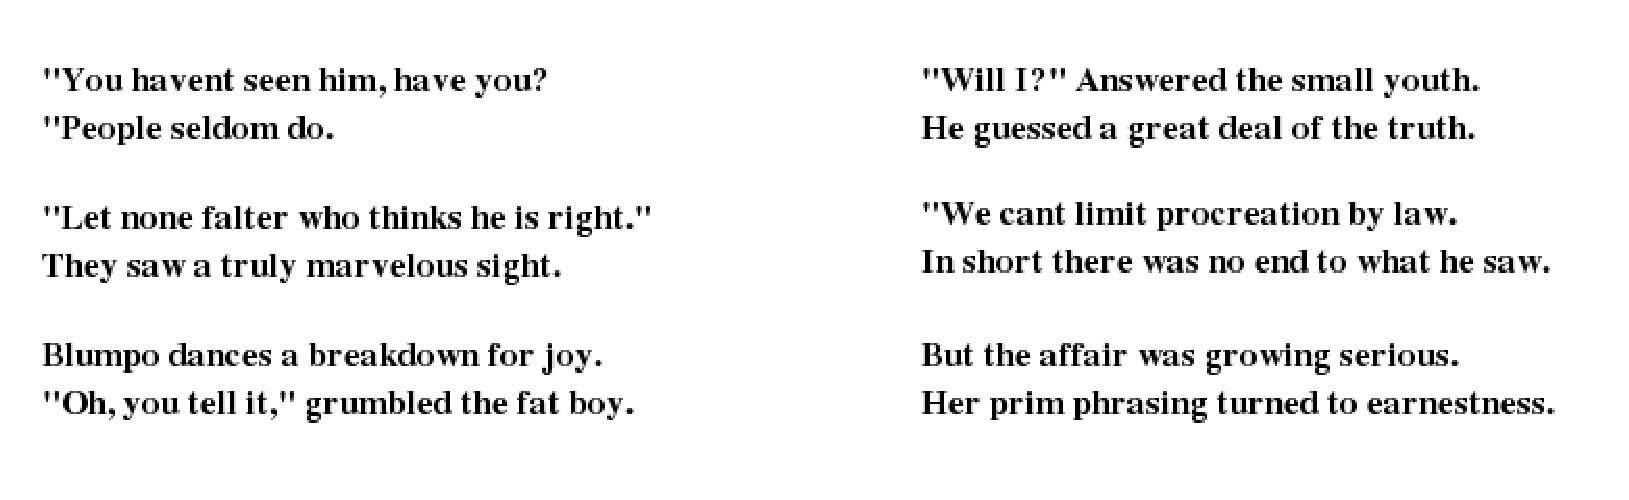
\includegraphics[width=5.5in]{couplets.eps}
\end{center}
\caption{Various couplets}
\end{figure}

Note the accidental semantic consistency in these pieces. Not only do the lines
often sound good together, it is easy for a reader to immediately find meaning
and coherence in the lines.

\subsubsection{Haiku}
Classic Haiku poems are 3 lines long with a 5-7-5 syllable pattern. Due to the
imprecise syllable counting the algorithm must often fall back on, the Haiku
presented here are not as strictly defined. However, they have the same look
and feel. They were generated with these guidelines:
\begin{verbatim}
--syllables="5,7,5" --length="3" 
\end{verbatim}

\begin{figure}[here]
\begin{center}
    \includegraphics[width=5.5in]{haiku.eps}
\end{center}
\caption{Various Haiku}
\label{fig:haiku}
\end{figure}

In these Haiku especially, one finds that many of the better poems are either
funny--jarring combinations of strange phrases--or oddly poignant. Of
particular note is the first haiku listed in \ref{fig:haiku}. One can imagine
a family staring out over the ruins of the Acropolis and pondering the
inevitable demise of Imperial glory.

\subsubsection{Limerick}
Limericks are typically obscene pieces beloning largely to folk traditions. The
algorithm was capable of producing limericks that traded obscenity for
absurdity. The rules used to generate the following were:

\begin{verbatim}
--rhyme="AABBA" --length="5" --syllables="10,10,6,6,10"
\end{verbatim}

\begin{figure}[here]
\begin{center}
    \includegraphics[width=5.5in]{limericks.eps}
\end{center}
\caption{Various limericks}
\label{fig:limericks}
\end{figure}

Given the line constraints it was difficult to produced topical limericks that
didn't weaken too much. But limericks of contrary absurdity were easy to come
by and seemed to fit the spirit of limericks anyway.

\subsubsection{Miscellaneous}

These pieces were created with a variety of inputs. Some are topically
oriented, others purely random. They were selected for their weight and
coherence.

\begin{figure}[here]
\begin{center}
    \includegraphics[width=6.5in]{misc.eps}
\end{center}
\caption{Various freeform works}
\label{fig:misc}
\end{figure}

Without syllable constraints, pieces end up with very long lines, as shown by
the indented line continuations in \ref{fig:misc}. Such lines, though, are
often poetic unto themselves and can work well within even a short piece. The
first piece listed in \ref{fig:misc} was made with the fuzzy keyword ``death''
and features a good mix of related and unrelated lines, sufficiently creating a
tone for the whole piece.

\subsection{Defense of Technique}

\subsubsection{Semantic Consistency}
By using one or more topics as rules in the input to the software one can
topically flavor the output without restricting it. Sentences relevant to the
selected topic will be used to produce the final piece. The reader should be
able to get a sense of what each produced poem is ``about.'' It is important to
note that this semantic consistency does not undermine juxtaposition, one of
the important aspects of computer poetry \cite{Hart96}. The output will still
contain the often jarring combination of seemingly otherwise unrelated phrases
despite their semantic consistency.

\subsubsection{Variable Structure}
Poems produced by my technique can scale from completely arbitrary, random
productions to very narrowly defined poetic structures (like sonnets, Haiku, or
limericks). The rules engine system allows for great flexibility and is a key
component of this technique. Its success, however, relies on the theory that
large enough corpora will contain sentences diverse enough to satisfy any input
rules.

\subsubsection{Human Mediated, Not Human Authored}
A key aspect of my approach is that, while all of the content used to produce
works is written by humans, the meaning of the content is subverted and altered
by the reappropriation process to create something new in which the humans and
computers involved both played integral roles in the poetic production. I refer
to the technique as being \emph{human mediated} as humans provide the
media--prose sentences--while the computer acts as the artist. In this case,
however, the computer is more like an artist of reappropriation like a DJ,
collage artist, or cut-up author.

\subsubsection{A Useful Seed}
Computer poetry can be a useful starting point for human poets, as noted in
\cite{Hart96}. This approach produces material that is easily reworked into a
more coherent piece by a discerning human artist. Often, merely changing just
one or two words in an output poem can make it match a particular scheme or
achieve some other poetic end.

\subsubsection{Conclusion}
Thus, I argue that this approach is a versatile one that employs the computer in a
necessary and novel way to produce interesting poetry. The rules system is
sufficiently `hands-off' such that a human merely suggests the final poetic
structure of a piece while the computer performs a task that is humanly
impossible. Thus, the `Why?' of this approach is: new, creative work is
discovered and enjoyed with the necessary help of a computer.

\section{Further Research}
\subsection{Missing Pieces}
The most glaring lacking in this implementation is the absence of a scansion
rule. Without this rule, most major poetic forms cannot be approximated. A
scansion engine\cite{scandroid} licensed under the GPL exists in the Python
language and could be adapted to work with the Perl source of this project.
Similarly, the current definition of rhyme used in this project is na\"{i}ve;
future iterations of this work will account for the many different kinds of
rhymes possible in a given poem (eg, syllabic, imperfect, or slant).

Further, I need to develop a faster way of acquiring and
profiling large corpora. It seems that refactoring and parallelizing parts of
the existing code would be the most expedient way to accomplish this.
Parallelization can also improve the production speed of longer poems with
several rules per line.

Finally, the resulting pieces need to be cleaned up in some automated
way--stray punctuation should be corrected, as should erroneous characters that
survived the profiling process (like newlines). Apostrophes, too, need to be
intelligently handled as for now they are just stripped out. As a part of this
project a Lingua::EN::Unapostrophe module was designed which would strip
possessive apostrophes but expand apostrophes representing word
contractions--from don't to do not, for example--but at time of publication the
design has not been implemented.

\subsection{Applications}
The quality of this approach's output depends largely on its corpus. Some areas
which would prove fruitful would be. One possible ``interesting'' corpus is a
mixture of the complete works of two poets, potentially radically different, to
create surprising combinations. Combining Plath and Whitman, for example, could
illustrate the often oscillating moods of self fulfillment and despair.
Similarly, news content from sources with different political agendas (eg, the
Huffington Post and the Drudge Report) could be combined to reveal excesses of
hyperbole on both sides of a political debate.

A more subtle application of this software is a kind of fuzzy data mining for
sociological research. The works produced by corpora containing every status
update of every friend of social network users from different socioeconomic
strata could elucidate differences in interests, literacy levels, and bias
between classes.

Finally, the entire Internet is a potential corpus; works
produced would seem infinitely diverse and could describe the zeitgeist of the
Internet's billions of users.

\bibliography{paper}
\bibliographystyle{apa}

\end{document}
